\chapter{Metodología propuesta}\label{chapter:proposal}

\section{Asimetría}

Como demuestran trabajos como \textit{3D-HGS} y \textit{Disc-GS}, abordar el problema de las discontinuidades en las superficies es fundamental para obtener mejores resultados de reconstrucción. Si bien enfoques como \textit{Convex Splatting}, \textit{DRK} y \textit{LinPrim} enfrentan este desafío mediante la modificación completa de la primitiva, ello conlleva incrementos considerables en el consumo de memoria y/o tiempo de cómputo, además de dificultar la integración de técnicas ya consolidadas sobre el framework original de \textit{Gaussian Splatting}. Por tal motivo, en este trabajo se propone utilizar la asimetría (\textit{skewness}) como mecanismo para resolver el problema, aprovechando que la función \textit{skew-normal} es una extensión natural de la función normal clásica. Esta función, al incorporar un parámetro de asimetría, permite modelar distribuciones con colas de diferente longitud y mayor flexibilidad, pero sin introducir una cantidad significativa de parámetros adicionales. Esto la hace especialmente adecuada para su implementación en \textit{pipelines} existentes.

\section{Simulación de la asimetría multivariante}

La forma propuesta de rasterizar una gaussiana con \textit{skewness} no reproduce técnicamente una función \textit{skew-normal} multivariante real, pero su comportamiento es análogo y cumple el mismo objetivo práctico, por lo que se hablará simplemente de asimetría en el contexto de este trabajo.

En la función \textit{skew-normal} en $\mathbb{R}^{3}$ se utilizan tres parámetros $\lambda$ que definen la dirección y magnitud de la asimetría. Para nuestra simulación se mantienen estos parámetros y, adicionalmente, se introduce un parámetro de sensibilidad $S$ que controla la nitidez del borde generado. Así, la nueva gaussiana rasterizada —siendo $A$ y $B$ dos gaussianas en $\mathbb{R}^{3}$ proyectadas a $\mathbb{R}^2$— se define mediante la siguiente fórmula:
\begin{equation}
    M = A \cdot (1 - e^{-S B})
    \label{eq:skew_mask}
\end{equation}
donde $B$ funciona como una máscara que determina la dirección del \textit{skewness} y define el borde duro. Específicamente, $B$ corresponde a la gaussiana $A$ trasladada por $\lambda$:
\[
B(x, y) = A\left(x - \lambda_x, y - \lambda_y\right)
\]
donde $\lambda \in \mathbb{R}^{2}$ es el vector de desplazamiento por \textit{skewness} en la imagen.

La elección de esta fórmula responde a la necesidad de crear un borde duro en un extremo de la primitiva y una cola suavizada en el otro. Visualmente, puede interpretarse como una pincelada que se desvanece: se genera una discontinuidad controlada en la opacidad, permitiendo tanto la creación de bordes definidos como la generación de gradientes o sombras del lado opuesto. Además, al estar compuesta únicamente por operaciones matemáticas básicas, la función resultante es diferenciable, lo que facilita su integración en flujos de trabajo optimizados y no requiere modificaciones profundas en el algoritmo de rasterización original.

\begin{figure}[htbp]
    \centering
    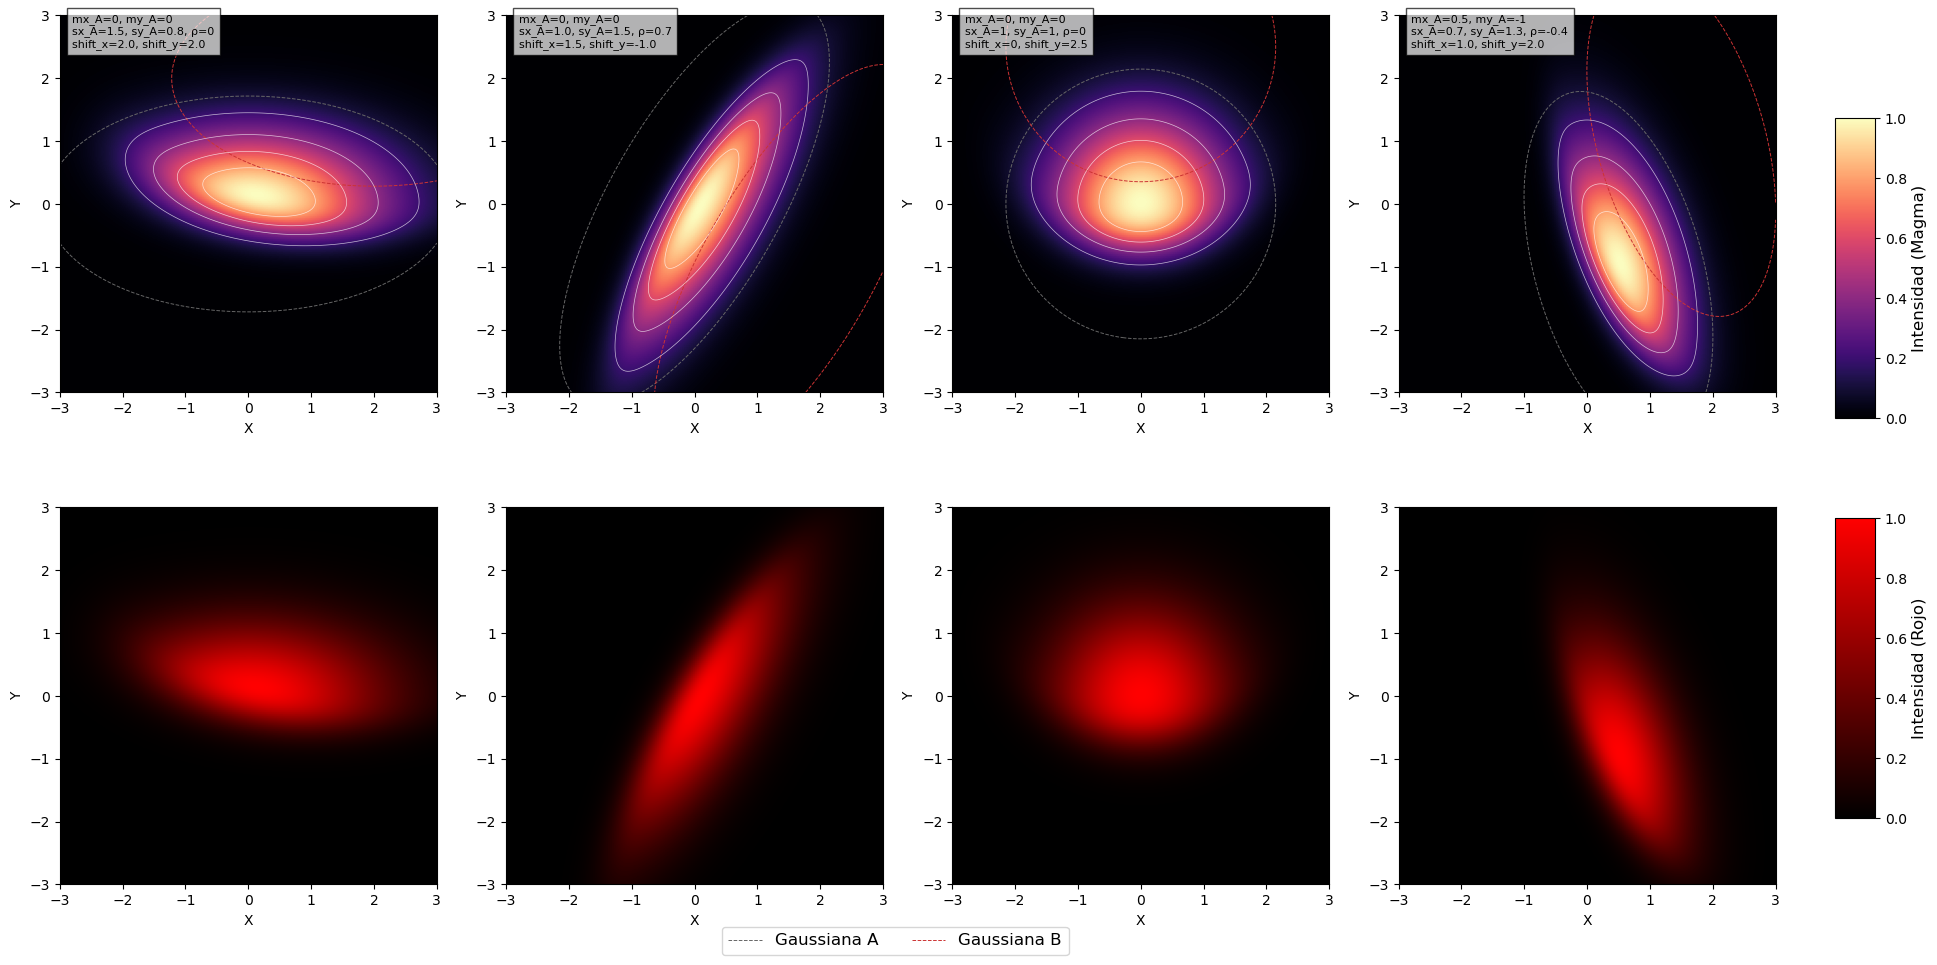
\includegraphics[width=1\textwidth]{Graphics/splatts.png}
    \caption{Visualización de la función de combinación \(A \cdot (1 - e^{-S B})\), utilizada para simular la asimetría. Se muestran cuatro configuraciones distintas de parámetros. La fila superior incluye mapas de calor con contornos de las gaussianas originales \(A\) y \(B\), mientras que la fila inferior muestra únicamente la distribución combinada en escala monocroma sobre fondo negro.}
    \label{fig:gaussianas_2d_skewness}
\end{figure}

Como $B$ es simplemente $A$ trasladada por $\lambda$, habiendo calculado:
\[
A_i(x, y) = \alpha_i^{\max} \exp\left(-\frac{1}{2}\mathbf{u}^{T}\mathbf{\Sigma}_i'^{-1}\mathbf{u}\right),
\]
siendo $\mathbf{u} = \begin{pmatrix} x \\ y \end{pmatrix} - \mathbf{x}_i$ y $\alpha_i^{\max}$ la opacidad máxima aprendida, sólo es necesario calcular además:
\[
B_i(x, y) = \exp\left(-\frac{1}{2}\mathbf{v}^{T}\mathbf{\Sigma}_i'^{-1}\mathbf{v}\right),
\]
donde $\mathbf{v} = \begin{pmatrix} x \\ y \end{pmatrix} - (\mathbf{x}_i - \lambda)$.
Posteriormente, se aplica la fórmula de combinación mediante la máscara:
\[
M_i(x, y) = A_i(x, y)\left[1 - \exp\left(-S B_i(x, y)\right)\right].
\]
El resto del algoritmo de rasterización se mantiene inalterado respecto a la versión clásica.

\section{Propagación de gradientes analítica}

Para implementar correctamente la optimización basada en gradientes, es necesario calcular de manera analítica las derivadas de la nueva función de máscara respecto a sus parámetros. Esto permite modificar el código de retropropagación (\textit{backward}) sin depender de aproximaciones numéricas.

\paragraph{Derivadas analíticas.}
%------------------------------------------------------------
%  Derivadas analíticas para el backward del “skew-splat”
%------------------------------------------------------------
\newcommand{\px}{x}\newcommand{\py}{y}
\newcommand{\dx}{d_x}\newcommand{\dy}{d_y}
\newcommand{\dlx}{d_x^{\lambda}}\newcommand{\dly}{d_y^{\lambda}}

\begin{align}
\mathbf{u} &= \begin{pmatrix}\px \\ \py\end{pmatrix}-\mathbf{x}_i,
&
\mathbf{v} &= \mathbf{u}-\boldsymbol{\lambda}_i,
\qquad
\boldsymbol{\lambda}_i=\begin{pmatrix}\lambda_{x,i}\\\lambda_{y,i}\end{pmatrix}
\\
A_i &= \alpha_i^{\max}\;
       \exp\!\Bigl(-\tfrac12\mathbf{u}^{\mathsf T}\mathbf{\Sigma}_i'\,\mathbf{u}\Bigr),
\label{eq:Adef}\\[2pt]
B_i &=       \exp\!\Bigl(-\tfrac12\mathbf{v}^{\mathsf T}\mathbf{\Sigma}_i'\,\mathbf{v}\Bigr),
\label{eq:Bdef}\\[2pt]
\alpha_i &= A_i\Bigl(1-e^{-S_i B_i}\Bigr).
\label{eq:alphadef}
\end{align}

%------------------------------------------------------------
\paragraph{Derivadas inmediatas de \(\alpha_i\)}%
\begin{align}
\frac{\partial\alpha_i}{\partial A_i} &= 1-e^{-S_i B_i},
&
\frac{\partial\alpha_i}{\partial B_i} &= A_i S_i e^{-S_i B_i},
&
\frac{\partial\alpha_i}{\partial S_i} &= A_i B_i e^{-S_i B_i}.
\label{eq:dalpha}
\end{align}

%------------------------------------------------------------
\paragraph{Derivadas de \(A_i\) }%
\begin{align}
\frac{\partial A_i}{\partial \alpha_i^{\max}}
  &= \frac{A_i}{\alpha_i^{\max}},
\\
\frac{\partial A_i}{\partial \Sigma'_{xx,i}}
  &= -\tfrac12\,\dx^{2}\,A_i,
&
\frac{\partial A_i}{\partial \Sigma'_{xy,i}}
  &= -\,\dx\dy\,A_i,
&
\frac{\partial A_i}{\partial \Sigma'_{yy,i}}
  &= -\tfrac12\,\dy^{2}\,A_i,
\\
\frac{\partial A_i}{\partial x_i}
  &= A_i\bigl(\Sigma'_{xx,i}\dx+\Sigma'_{xy,i}\dy\bigr),
&
\frac{\partial A_i}{\partial y_i}
  &= A_i\bigl(\Sigma'_{xy,i}\dx+\Sigma'_{yy,i}\dy\bigr).
\label{eq:dA}
\end{align}

%------------------------------------------------------------
\paragraph{Derivadas de \(B_i\)}%
\[
\dlx=\dx-\lambda_{x,i},\qquad
\dly=\dy-\lambda_{y,i}
\]

\begin{align}
\frac{\partial B_i}{\partial \Sigma'_{xx,i}}
  &= -\tfrac12\,\dlx^{2}\,B_i,
&
\frac{\partial B_i}{\partial \Sigma'_{xy,i}}
  &= -\,\dlx\dly\,B_i,
&
\frac{\partial B_i}{\partial \Sigma'_{yy,i}}
  &= -\tfrac12\,\dly^{2}\,B_i,
\\
\frac{\partial B_i}{\partial \lambda_{x,i}}
  &=  B_i\bigl(\Sigma'_{xx,i}\dlx+\Sigma'_{xy,i}\dly\bigr),
&
\frac{\partial B_i}{\partial \lambda_{y,i}}
  &=  B_i\bigl(\Sigma'_{xy,i}\dlx+\Sigma'_{yy,i}\dly\bigr),
\\
\frac{\partial B_i}{\partial x_i}
  &= -B_i\bigl(\Sigma'_{xx,i}\dlx+\Sigma'_{xy,i}\dly\bigr),
&
\frac{\partial B_i}{\partial y_i}
  &= -B_i\bigl(\Sigma'_{xy,i}\dlx+\Sigma'_{yy,i}\dly\bigr).
\label{eq:dB}
\end{align}

%------------------------------------------------------------
\paragraph{Derivada de la pérdida respecto a \(\alpha_i\)}

Para cada píxel \(p\) (y canal \(c\)), definimos la transmitancia
\(
T_{i-1,p}= \prod_{j<i}\bigl(1-\alpha_{j,p}\bigr)
\)
y el color acumulado antes de la primitiva \(i\) como
\(C_{p,c}^{\text{prev}}\).
Sea
\(g_{p,c}= \partial\mathcal{L}/\partial C_{p,c}\)
y, si se usa la regularización por profundidad,
\(h_p=\partial\mathcal{L}/\partial D_p\).
Entonces
\[
\frac{\partial\mathcal{L}}{\partial \alpha_{i,p}}
  =T_{i-1,p}\!\left[
      \sum_{c=1}^{C}\bigl(f_{i,c}-C_{p,c}^{\text{prev}}\bigr)g_{p,c}
      \;+\;
      \bigl(\tfrac1{d_i}-D_{p}^{\text{prev}}\bigr)h_{p}
    \right].
\label{eq:dLdalpha}
\]

Luego utilizando la regla de la cadena:

\begin{align}
\frac{\partial\mathcal{L}}{\partial f_{i,c}}
  &= \sum_{p}T_{i-1,p}\,\alpha_{i,p}\,g_{p,c},
\\
\frac{\partial\mathcal{L}}{\partial \alpha_i^{\max}}
  &=\sum_{p}
     \frac{\partial\mathcal{L}}{\partial\alpha_{i,p}}\;
     (1-e^{-S_i B_{i,p}})\,
     \frac{A_{i,p}}{\alpha_i^{\max}},
\\
\frac{\partial\mathcal{L}}{\partial S_i}
  &=\sum_{p}
     \frac{\partial\mathcal{L}}{\partial\alpha_{i,p}}\;
     A_{i,p} B_{i,p} e^{-S_i B_{i,p}},
\\
\frac{\partial\mathcal{L}}{\partial \lambda_{x,i}}
  &=\sum_{p}
     \frac{\partial\mathcal{L}}{\partial\alpha_{i,p}}\;
     A_{i,p}S_i e^{-S_i B_{i,p}}\,B_{i,p}\,
     \bigl(\Sigma'_{xx,i}\dlx+\Sigma'_{xy,i}\dly\bigr),
\end{align}

y análogamente para \(\lambda_{y,i}\),
los tres elementos \(\Sigma'_{xx,i},\Sigma'_{xy,i},\Sigma'_{yy,i}\)
y las coordenadas \(x_i,y_i\).



\section{Complejidad computacional y análisis de estabilidad numérica}

\subsection{Comparación de complejidad computacional}

El método propuesto introduce una ligera modificación sobre el \textit{Gaussian Splatting} clásico, pero mantiene la misma complejidad asintótica global. En el proceso de rasterización, mientras que el método clásico requiere únicamente una evaluación exponencial por cada píxel afectado (correspondiente a la gaussiana original), la versión con máscara \textit{skew} exige tres evaluaciones exponenciales por píxel: dos para las gaussianas $A$ y $B$ y una adicional para calcular la función de unión $1 - e^{-SB}$. Sin embargo, todas estas operaciones pueden fusionarse en un mismo núcleo de cálculo (\textit{kernel}), por lo que la penalización computacional resulta en un simple factor constante, típicamente en el rango de $1.8$ a $2.5$ veces el costo original en términos de operaciones de punto flotante (\textit{FLOPs}).

El resto de las etapas del algoritmo, incluyendo la composición alfa de los píxeles y la acumulación de resultados, se mantiene inalterado respecto al método clásico. Durante la fase de propagación de gradientes, se añaden derivadas respecto a los nuevos parámetros ($S$ y $\lambda$), pero el cálculo sigue siendo local y de complejidad constante por primitiva. Así, la complejidad global se mantiene en $O(Nk)$, donde $N$ es el número de primitivas gaussianas y $k$ el número de píxeles afectados por cada una.

En cuanto al consumo de memoria, la adición de los parámetros $S$ (sensibilidad) y $\lambda$ (vector de \textit{skewness}) implica un aumento marginal, ya que representan apenas cuatro números de punto flotante adicionales por cada primitiva. Este incremento suele ser despreciable en comparación con el resto de los atributos asociados a cada splat, como las texturas de armónicos esféricos.


\subsection{Estabilidad numérica de la modificación}

Al extender la formulación clásica con la máscara $A(1-e^{-SB})$, surgen algunas consideraciones sobre la estabilidad numérica de la implementación. En primer lugar, la función exponencial puede producir valores extremadamente pequeños cuando el argumento $SB$ es grande, lo que puede causar problemas de \textit{underflow} y anular los gradientes en regiones de opacidad muy alta. Para mitigar este efecto, se limitan los valores máximos de $S$ y se trabaja con precisión flotante simple (FP32).

En el extremo opuesto, cuando $SB$ es muy pequeño, la resta $1-e^{-SB}$ puede provocar cancelación numérica y pérdida de precisión, manifestándose en artefactos visuales de banda fina en los bordes de las primitivas. Este problema se evita reemplazando la operación por la función estándar \texttt{expm1}.

Otro posible inconveniente es la aparición de gradientes de gran magnitud, especialmente si $S$ crece sin restricciones, lo que puede desestabilizar el proceso de optimización durante el entrenamiento. Para mantener la estabilidad,se restringe el rango de $S$ mediante una función sigmoide acotada

Finalmente, como en el método clásico, es fundamental evitar que la matriz de covarianza $\Sigma$ adquiera valores demasiado pequeños, ya que esto puede provocar divisiones por casi cero y la aparición de “píxeles calientes” que dominan la función de pérdida. Esta situación se controla limitando los valores propios mínimos de $\Sigma$.

